%!TEX root = final.tex
\newpage
\appendix
\section{Appendix} \label{appendixA}
Below we provide further details including confusion matrices and
reliability plots on some of the models used.

\begin{figure}[h]
  \centering
    \begin{subfigure}[p!]{\textwidth}
            \caption{Non--Quality of Life Cases}
            \begin{subfigure}[p!]{0.49\textwidth}
              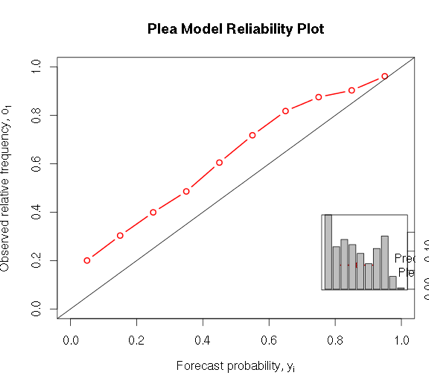
\includegraphics[width=\textwidth]{figures/appa.png}
              \label{fig:AppA}
            \end{subfigure}
            ~
            \begin{subfigure}[p!]{0.49\textwidth}
              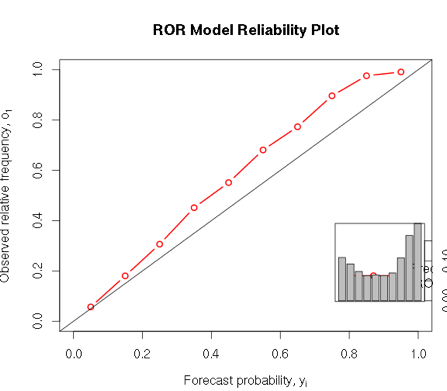
\includegraphics[width=\textwidth]{figures/appb.png}
              \label{fig:AppB}
            \end{subfigure}
    \end{subfigure}

    \begin{subfigure}[p!]{\textwidth}
                \caption{Quality of Life Cases}
                \begin{subfigure}[p!]{0.49\textwidth}

                  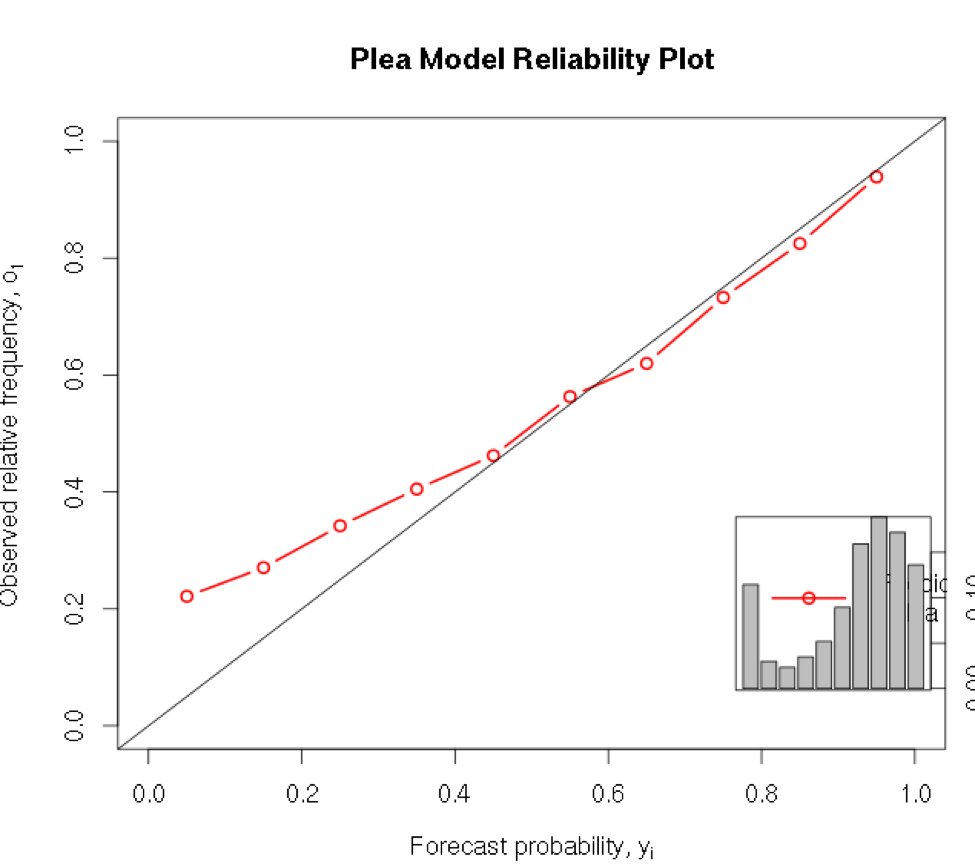
\includegraphics[width=\textwidth]{figures/appc.png}
                  \label{fig:AppC}
                \end{subfigure}
                ~
                \begin{subfigure}[p!]{0.49\textwidth}

                  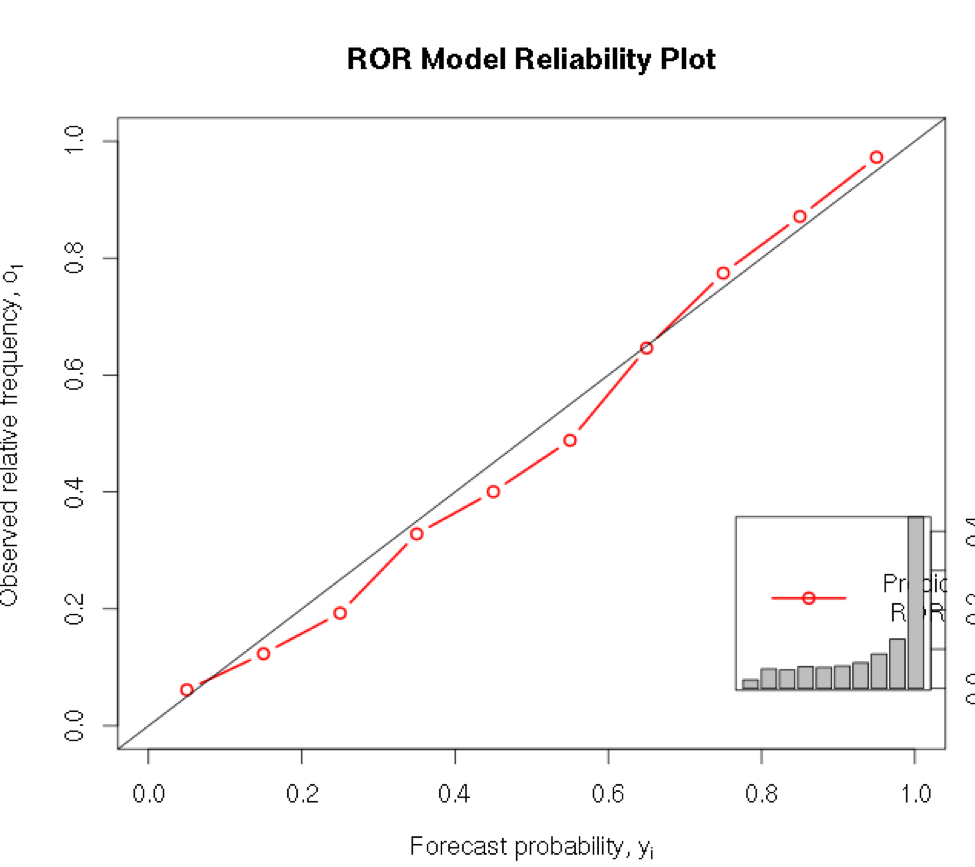
\includegraphics[width=\textwidth]{figures/appd.png}
                  \label{fig:AppD}
                \end{subfigure}
      \end{subfigure}
      \caption{Random Forest Model}
\end{figure}
\newpage

\begin{figure}[h]
  \centering
    \begin{subfigure}[p!]{\textwidth}
    \caption{ROR Modeling using GLM}
        \begin{subfigure}[p1]{0.49\textwidth}
            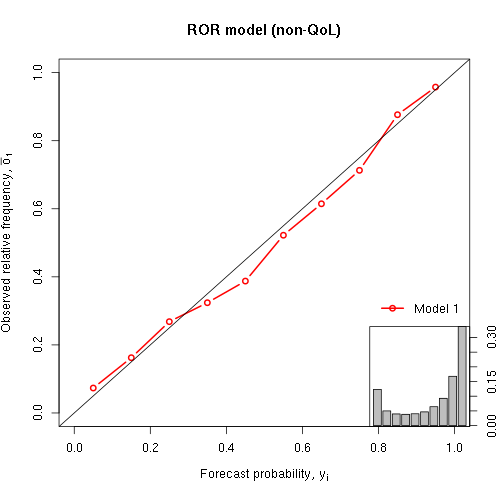
\includegraphics[width=\textwidth]{figures/glmplots/ror_fc.png}
        \end{subfigure}
        ~
        \begin{subfigure}[p1]{0.49\textwidth}
            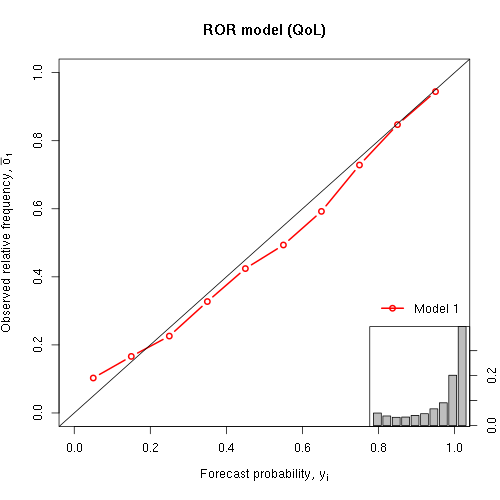
\includegraphics[width=\textwidth]{figures/glmplots/rorq_fc.png}
        \end{subfigure}
    \end{subfigure}


    \begin{subfigure}[p!]{\textwidth}
    \caption{Plea Rates Modeled using GLM}
        \begin{subfigure}[p1]{0.49\textwidth}
            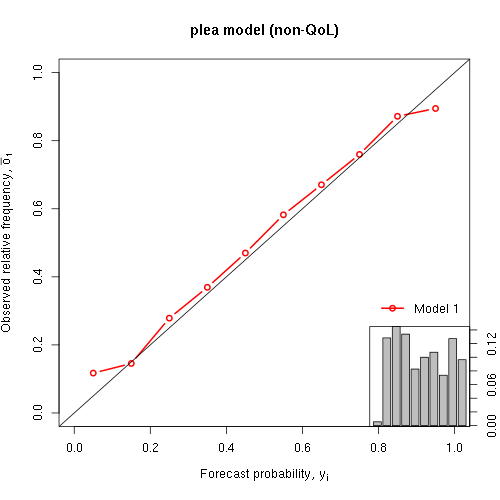
\includegraphics[width=\textwidth]{figures/glmplots/plea_fc.png}

        \end{subfigure}
        ~
        \begin{subfigure}[p1]{0.49\textwidth}
            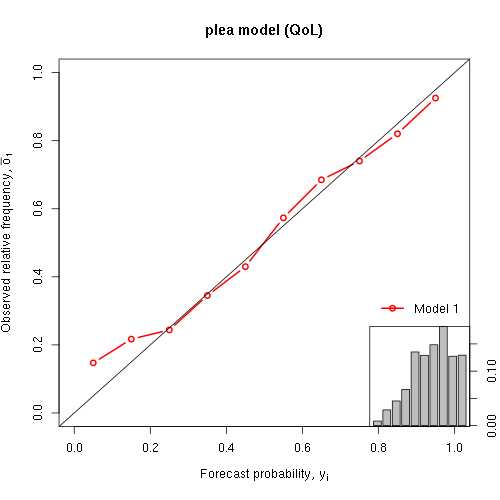
\includegraphics[width=\textwidth]{figures/glmplots/pleaq_fc.png}

        \end{subfigure}
    \end{subfigure}

\end{figure}

\subsection{Validating GLM}
With a half and half test/train split,
the ROR model had acceptable performance,
while the plea model's performance was rather unremarkable.
Though their accuracy rates are not abysmal,
it is important to keep in mind that
both outcomes being predicted have relatively high frequency in the data
(ROR rate is close to 65 percent and plea rate is around 50 percent).